\documentclass[conference,a4paper]{IEEEtran}

\usepackage{cite}
\usepackage{graphicx}

\begin{document}

\title{A secondary screen architecture to accurately capture TV viewer interactions for content personalization in TV environments}

\author{\IEEEauthorblockN{Ricardo E. V. de S. Rosa}
\IEEEauthorblockA{Graduate Program in Electrical Engineering \\ Federal University of Minas Gerais \\ Av. Antônio Carlos 6627, 31270-901, \\Belo Horizonte, MG, Brazil\\
Email: ricardoerikson@ufmg.br}
\and
\IEEEauthorblockN{Vicente F. de Lucena Junior}
\IEEEauthorblockA{Graduate Program in Electrical Engineering \\
Federal University of Amazonas \\
Manaus, AM, Brazil\\
Email: vicente@ufam.edu.br}
}
\maketitle

\begin{abstract}
TV watching is frequently seen as a social activity. People gather around the television for entertainment or information. Advances in TV technology have enabled the viewer to actively interact with applications and providers instead of just passively watch TV. One important application for the viewers is content personalization, which consists in generating content recommendations based on viewers' interactions. Since the TV set is shared by many people, it is difficult to accurately capture the individual interactions from every viewer using a traditional remote control. In this paper, we present an architecture that facilitates the identification of viewers and the capture of their individual interactions in shared TV environments.
\end{abstract}

\IEEEpeerreviewmaketitle

\section{Introduction}

TV watching is essentially a social activity, where family, friends, or people with a common interest share the same space and TV set for entertainment or information~\cite{Masthoff2004}. After many advances in technologies for interactive and digital TV it is possible to develop high level applications to enrich the TV experience. Thus, the interaction between viewers and TV became more elaborated than simply change channel and volume.

The interactions between viewers and TV can be classified as implicit and explicit. Implicit interactions are part of the natural actions of watching TV e.g., change channel and volume. In explicit interactions viewers contribute by actively evaluating, commenting or sharing their opinion about a given content. Both kinds of interaction are important for applications that rely on audience generated data.

Considering the interactions of millions of viewers, the captured data can provide valuable information~\cite{Teixeira2010}. For example, the content providers (CP) can obtain the user ratings given to TV programs, amount of viewers and user profiles. One important application that makes use of viewers interaction is content personalization. Content providers can infer user profiles from viewers' interactions in order to deliver personalized content.

The traditional remote control (RC) is the input device that viewers typically use to interact with the TV. However, the RC presents two notable problems for capturing interactions from viewers: (1) to automatically identify the viewers in the TV environment; and (2) to individually capture interactions of the viewer in charge of the RC. Thus, considering a scenario with the traditional RC, all interactions are assigned to the whole group of viewers (e.g., a family), rather than to the viewer in charge of the RC. As a result, the tastes that were inferred from the users in charge of the RC can be imposed on the tastes of others.

As a potential mean to handle the limitations of the RC for capturing interactions from viewers, the proliferation of personal mobile devices has changed the people behavior towards audiovisual content consumption in interactive TV environments. Nowadays, viewers rarely just sit passively and watch TV. In many situations they use their personal devices as a secondary screen to perform activities related to TV watching, which end up enriching and immersing the user into the TV experience. 

Secondary screen devices arise as a powerful mechanism to accurately identify viewers and  capture their interactions. In this research field, a typical approach is to use personal devices (e.g., smartphones and tablets) as secondary screens~\cite{Courtois2012}, since they are almost ubiquitous and present good graphical capabilities and Internet connection. The connectivity capabilities of smartphones were used in~\cite{Cabarcos2011}, where the Bluetooth technology was used to detect nearby users. With respect to interaction capture, an approach described in~\cite{Teixeira2010} shown an architecture to capture contextualized viewers interactions through a conventional remote control. In this paper, we present an architecture that enables identifying viewers and capturing their interactions using a personal device as secondary screen. 

\section{Architecture}

This architecture consists of secondary screen devices (which might be implemented in personal devices such as smartphones and tablets) a set-top box (STB) with return channel, and a CP (which is responsible for providing the interactive applications and for storing the data that is captured from viewers).

Initially, the CP must provide an infrastructure for viewers and the STB so that they can be authenticated to use the application services. In addition, the infrastructure must also provide data storage capabilities to store the interaction data captured from viewers. Then the STB must be authenticated in the application hosted on the CP infrastructure. Once the STB is authenticated, the viewers in the TV environment must also authenticate in the application service and register the STB in their accounts. As a result, the viewer can use their personal device as a secondary screen for that STB.

Figure~\ref{fig_architecture} Green arrows represent data flowing from the viewer to the CP infrastructure, while blue arrows represent the flow from CP to viewer. The black arrows represent data flow inside the CP infrastructure.

The secondary screen device must be used in conjunction with the STB to identify the users that are present in the environment and update context information. In the first place, the STB 

That is, the viewer can authenticate to the local set-top box by using a transparent authentication mechanism. Thus, every time a viewer is nearby the STB using a a TV application with its 

The second screen devices are Internet capable devices, which have TV related applications. The viewers use these applications to interact with the TV by evaluating, commenting or sharing TV content.

\begin{figure}[!t]
	\centering
	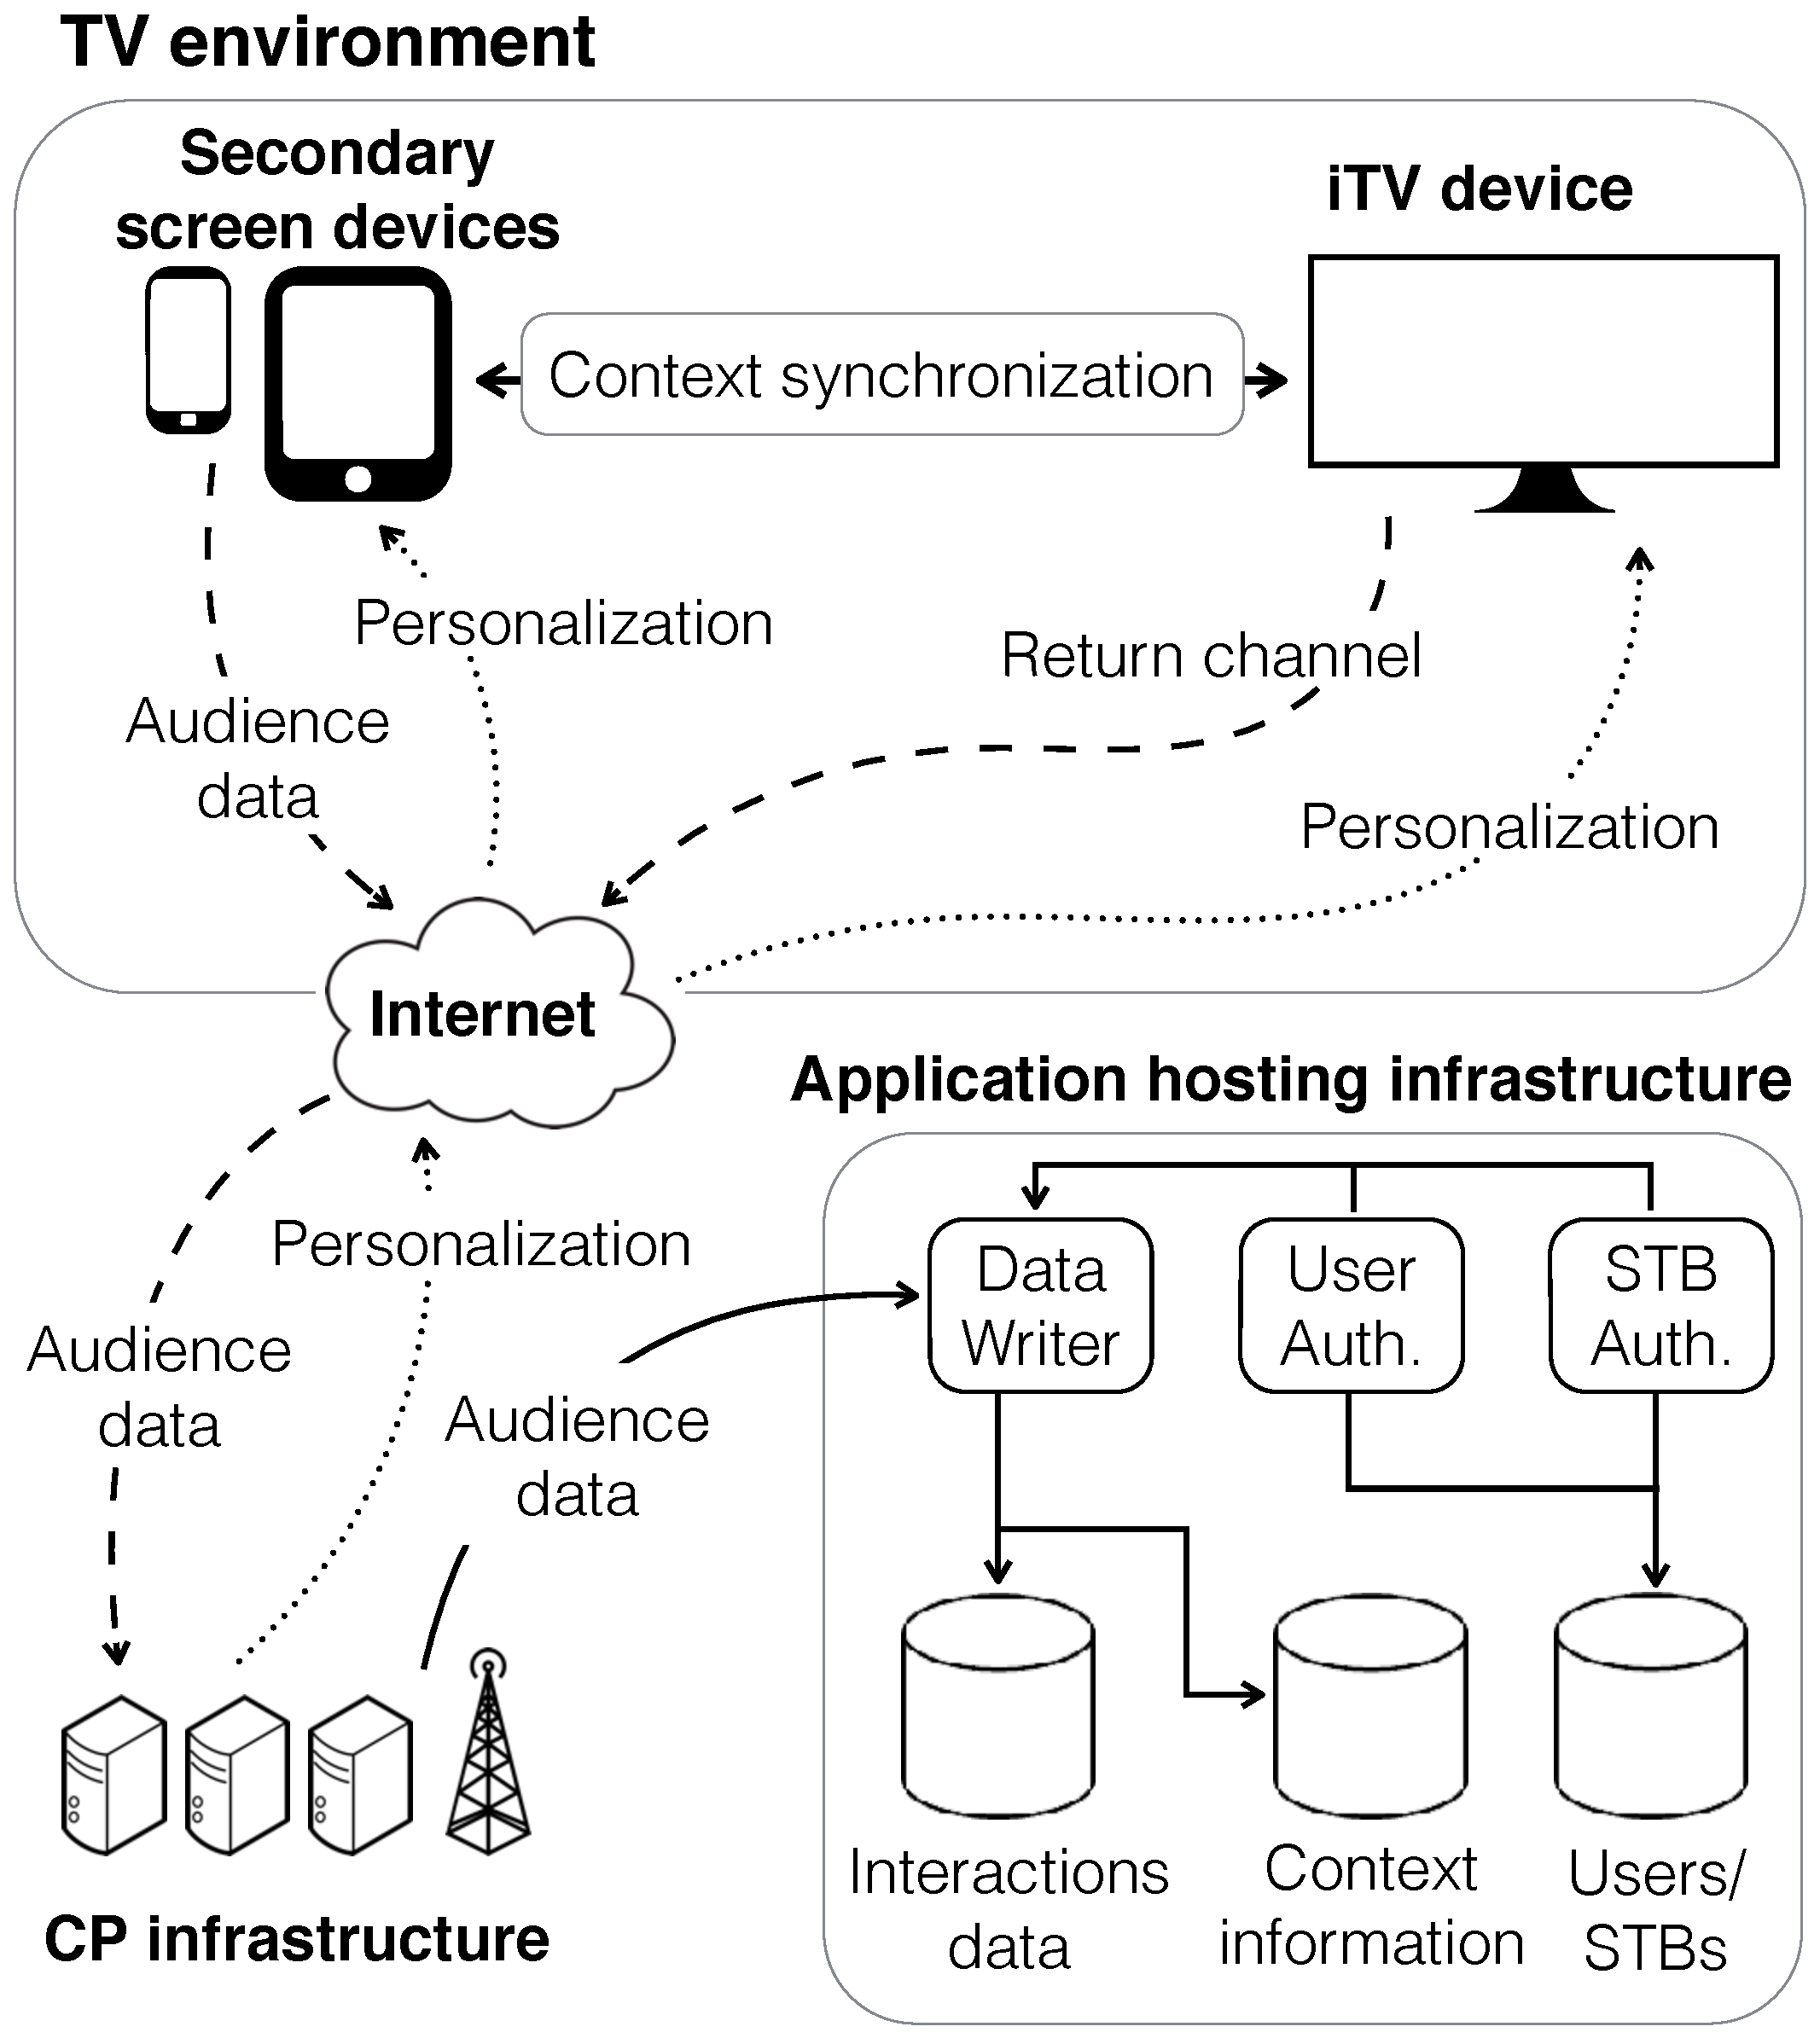
\includegraphics[width=3.5in]{img/architecture.pdf}
	\caption{Architecture to capture viewers insteractions. }
	\label{fig_architecture}
\end{figure}

The STB is synchronized with the TV in order to contextualize the data that is captured.
\cite{Lee2010}

\section{Conclusions}

Since applications in the TV domain have potential to deal with millions of users at the same time, it is interesting that this infrastructure has the ability to handle a growing amount of data~\cite{Lee2010}.

\bibliographystyle{IEEEtran}
\bibliography{biblio.bib}

\end{document}


